\documentclass[10pt]{article}
\usepackage[usenames]{color} %used for font color
\usepackage{amssymb} %maths
\usepackage{amsmath} %maths
\usepackage{bbold} % indicators
\usepackage[utf8]{inputenc} %useful to type directly diacritic characters
\usepackage{tikz}
\begin{document}
\[
  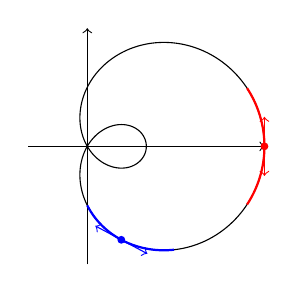
\begin{tikzpicture}[scale=3/4]
    \draw[->] (0, -2) -- (0, 2);
    \draw[->] (-1, 0) -- (3, 0);
    \draw[domain=0:360,smooth,variable=\t,samples=360]
      plot ({cos(\t) * (1 + 2 * cos(\t))},{sin(\t) * (1 + 2 * cos(\t))});
    \draw[domain=-20:20,smooth,variable=\t,color=red, thick,samples=40]
      plot ({cos(\t) * (1 + 2 * cos(\t))},{sin(\t) * (1 + 2 * cos(\t))});
    \draw[domain=270:310,smooth,variable=\t,color=blue, thick,samples=40]
      plot ({cos(\t) * (1 + 2 * cos(\t))},{sin(\t) * (1 + 2 * cos(\t))});
    \draw[<->, color = red] (3, -1/2) --
      node [midway, circle, fill = red, inner sep = 1pt] {} (3, 1/2);
    \draw[<->, color = blue] (0.135, -1.347) --
      node[midway, circle, fill = blue, inner sep = 1pt] {} (1.017, -1.818);
  \end{tikzpicture}
\]
\end{document}
